\chapter{Theory}
This chapter is going to explain the theories behind the techniques used for this project. Each technique will be elaborated and explain when and how it is being used.
\section{Image Processing}
During this project a lot of image processing has been used. The different image processing techniques are used in a combination to display exactly what we want to output. Some techniques is being used to remove noise from the picture so the important parts gets all the focus, while others are used for making the important parts more clear or making it possible to track specific parts of the output. \\
It is all these different techniques combined that makes it possible to get a functional product, but before you can use them, you will have to know how they work and how they can be included to your project. This section is going to explain the different techniques that are being used and also why and how they are being used in this project.
\subsection{Threshold}
Threshold is one of the most fundamental operations in point processing and is used to take an input picture and make it binary. Making an image binary means to show the image in only completely black and completely white pixel values. \\
This function could be useful in programs where you need to find silhouettes, tracking a person for example, and smaller details are not as important. \\
To determine which pixels that should be completely black and which should be completely white a threshold value is required. The threshold value can be compared to a gatekeeper who lets everyone who is 18 years old or older inside the club, but denies everyone who is 17 years old or younger. However with threshold getting in equals to becoming a white pixel and getting denied equals to a black pixel if the chosen threshold value was 18 like in this example. To sum this up the formula for making a threshold is shown below:
\begin{equation}
  \begin{aligned}
  	\text{if } f(x,y)\leq T \quad \text{then } g(x,y)=0 \\
  	\text{if } f(x,y)>T \quad \text{then } g(x,y)=255
  \end{aligned} 
\end{equation}
Where $T$ is the threshold value, $f(x,y)$ is the input pixel and $g(x,y)$ is the output pixel. 

When choosing the threshold value it is important to think about what the wanted output is. It differs a lot from picture to picture how effective threshold is based on the difference between the object and the background. If the background and the object you want to find is very different in color then it is easy to distinguish between them and choose an effective threshold value. However if the object and background is very similar then it becomes a lot harder since you will have to chose between losing some information from the wanted object to remove background noise, or keep the object clear but have more background noise. \\
To get a better understanding of this look at the two histograms below showing the histograms of two grey-scale pictures. It is easy to tell that the leftmost histogram \eqref{fig:SimpleThreshold} is more ideal to threshold because the object and background are very different while the rightmost histogram \eqref{fig:ComplicatedThreshold} has very similar object and backgrounds.

\begin{figure}[htbp] \centering
\begin{minipage}[b]{0.45\textwidth} \centering
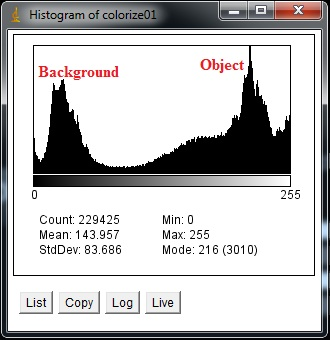
\includegraphics[width=1.00\textwidth]{Pictures/Theory/SimpleThresholdPicture} % Venstre billede
\end{minipage} \hfill
\begin{minipage}[b]{0.45\textwidth} \centering
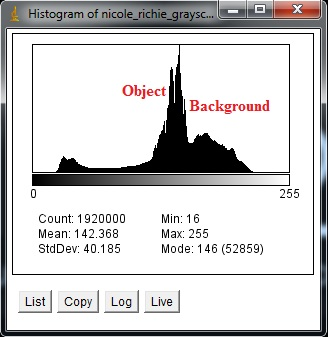
\includegraphics[width=1.00\textwidth]{Pictures/Theory/ComplicatedThresholdPicture} % Højre billede
\end{minipage} \\ % Captions og labels
\begin{minipage}[t]{0.45\textwidth}
\caption{Simple threshold value} % Venstre caption og label
\label{fig:SimpleThreshold}
\end{minipage} \hfill
\begin{minipage}[t]{0.45\textwidth}
\caption{Complicated threshold value} % Højre caption og label
\label{fig:ComplicatedThreshold}
\end{minipage}
\end{figure}

The first picture which had the leftmost histogram can be seen on image \eqref{fig:SimpleThresholdAfter} and shows that after using threshold it makes a nice silhouette of the woman. However the picture from the rightmost histogram gets a very poor silhouette of a woman because the background and the woman has almost the same color. This can be seen on image \eqref{fig:ComplicatedThresholdAfter} which shows the picture after using threshold.

\begin{figure}[htbp] \centering
\begin{minipage}[b]{0.45\textwidth} \centering
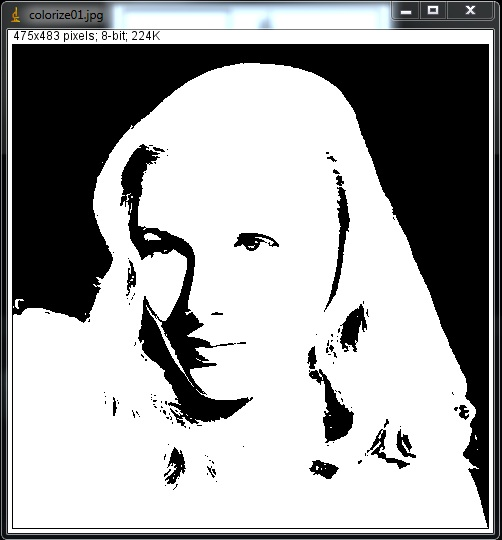
\includegraphics[width=1.00\textwidth]{Pictures/Theory/SimpleThresholdAfter} % Venstre billede
\end{minipage} \hfill
\begin{minipage}[b]{0.45\textwidth} \centering
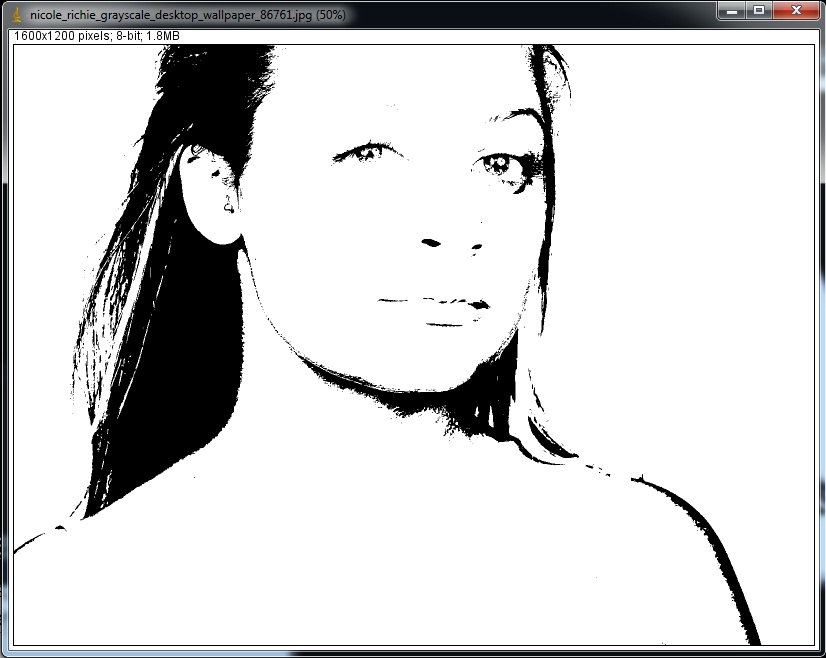
\includegraphics[width=1.00\textwidth]{Pictures/Theory/ComplicatedThresholdAfter} % Højre billede
\end{minipage} \\ % Captions og labels
\begin{minipage}[t]{0.45\textwidth}
\caption{Great silhouette after threshold} % Venstre caption og label
\label{fig:SimpleThresholdAfter}
\end{minipage} \hfill
\begin{minipage}[t]{0.45\textwidth}
\caption{Bad silhouette after threshold} % Højre caption og label
\label{fig:ComplicatedThresholdAfter}
\end{minipage}
\end{figure}
 
 
 
\subsection{Morphology}
\subsubsection{Hit}
\subsubsection{Fit}
\subsubsection{Dilation}
\subsubsection{Erosion}
\subsubsection{Opening}
\subsection{BLOB-Analysis}
The term BLOB stands for Binary Large Objects and refers to a region of connected pixels in a binary image. Therefore, this technique is used to extract meaningful information from images.
A common problem when dealing with images is to determine if the image data contains a particular object or shape, by detecting points or regions that differ in properties like brightness or color changes.
\subsubsection{Grass Fire}
\subsubsection{BLOB Classification}

